\documentclass[a4paper,12pt]{article}
\usepackage[brazil]{babel}
\usepackage[utf8]{inputenc}
\usepackage[T1]{fontenc}
\usepackage{geometry}
\usepackage{setspace}
\usepackage{titlesec}
\usepackage{hyperref}
\usepackage{graphicx}
\usepackage{caption}
\usepackage{subcaption}
\usepackage{fancyhdr}
\usepackage{xcolor}
\usepackage{xcolor}
\usepackage{amsmath}
\usepackage{tikz}

\input{commands.tex}

\hypersetup{
    colorlinks=true,% make the links colored
    linkcolor=blue
}

\usepackage{setspace}
\addbibresource{bibliography.bib}

\newcommand{\printingbibliography}{%

    \pagestyle{myheadings}
    \markright{}
    \sloppy
    \printbibliography[heading=bibintoc, % add to table of contents
                   title=Refer\^encias % Chapter name
                  ]
    \fussy%
}
\PassOptionsToPackage{table}{xcolor}
\renewcommand{\baselinestretch}{1.5}

\pagestyle{fancy}
\fancyhf{}
\renewcommand{\headrulewidth}{1pt}
\fancyhead[R]{\thepage}

\geometry{a4paper,top=30mm,bottom=20mm,left=30mm,right=20mm}

\titleformat*{\section}{\bfseries\large}
\titleformat*{\subsection}{\bfseries\normalsize}

\rhead{Guia de Estudo - Física - 1ª Série EM}
\lhead{Prof. André Vieira da Silva}
\rfoot{\thepage}

\title{\textbf{Guia de Estudo \\Física - 1ª Série do Ensino Médio}}
\author{Prof. André Vieira da Silva}
\date{}
\date{\today}

\begin{document}

\maketitle
\tableofcontents
\newpage

%==================================================
\section{Cinemática}

\subsection{Conceitos Fundamentais}
A cinemática é a parte da Física que estuda os movimentos sem se preocupar com suas causas.  
Os principais conceitos são:

\begin{itemize}
    \item \textbf{Referencial:} ponto de vista a partir do qual se observa o movimento.
    \item \textbf{Posição ($s$):} local onde o corpo se encontra.
    \item \textbf{Deslocamento ($\Delta s$):} variação da posição: $\Delta s = s - s_0$.
    \item \textbf{Velocidade média:} $v_m = \dfrac{\Delta s}{\Delta t}$.
    \item \textbf{Aceleração média:} $a_m = \dfrac{\Delta v}{\Delta t}$.
\end{itemize}

\subsection{Movimento Uniforme (MU)}
No MU a velocidade é constante:
\[
s = s_0 + vt
\]

\textbf{Exemplo:} Um carro parte do km 10 e viaja a 90 km/h.  
Após 2 horas, sua posição será:
\[
s = 10 + 90 \times 2 = 190 \text{ km}
\]

\subsection{Movimento Uniformemente Variado (MUV)}
A aceleração é constante:
\[
v = v_0 + at \qquad \text{e} \qquad s = s_0 + v_0t + \frac{at^2}{2}
\]
A equação de Torricelli relaciona $v$, $v_0$, $a$ e $\Delta s$:
\[
v^2 = v_0^2 + 2a\Delta s
\]

\textbf{Exemplo:} Um carro acelera de $10\,m/s$ para $20\,m/s$ em 5 s:
\[
a = \frac{20 - 10}{5} = 2\,m/s^2
\]

\subsection{Exercícios}
\subsubsection{Um móvel parte do repouso e percorre $100\,m$ em $10\,s$. Determine a aceleração.}
{\color{blue}
\textbf{Resolução:}

Sabemos que:
\[
v_0 = 0 \quad ; \quad \Delta s = 100\,m \quad ; \quad t = 10\,s
\]

Utilizamos a equação do movimento uniformemente variado:
\[
\Delta s = v_0 t + \frac{1}{2} a t^2
\]

Substituindo os valores:
\[
100 = 0 \cdot 10 + \frac{1}{2} a (10)^2
\]

\[
100 = \frac{1}{2} a \cdot 100
\]

\[
100 = 50a
\]

\[
a = \frac{100}{50}
\]

\[
a = 2\,m/s^2
\]

\textbf{Resposta:} $a = 2\,m/s^2$
}

\newpage

\subsubsection{Um carro a $72\,km/h$ percorre 150 km. Calcule o tempo gasto.}

{\color{blue}
\textbf{Resolução:}

Dados:
\[
v = 72\,km/h \quad ; \quad \Delta s = 150\,km
\]

Usamos:
\[
v = \frac{\Delta s}{t}
\]

Isolando o tempo:
\[
t = \frac{\Delta s}{v}
\]

Substituindo:
\[
t = \frac{150}{72}
\]

\[
t \approx 2{,}08\,h
\]

Convertendo a parte decimal:
\[
0{,}08 \times 60 \approx 5\,min
\]

\[
t \approx 2\,h \; 5\,min
\]

\textbf{Resposta:} $t \approx 2\,h \; 5\,min$

}

\newpage

\subsubsection{Um corpo com $v_0 = 5\,m/s$ e $a = 2\,m/s^2$ encontra sua velocidade após 6 s.}

{\color{blue}
\textbf{Resolução:}

Dados:
\[
v_0 = 5\,m/s \quad ; \quad a = 2\,m/s^2 \quad ; \quad t = 6\,s
\]

Equação da velocidade no MUV:
\[
v = v_0 + a t
\]

Substituindo:
\[
v = 5 + 2 \cdot 6
\]

\[
v = 5 + 12
\]

\[
v = 17\,m/s
\]

\textbf{Resposta:} $v = 17\,m/s$

}

\newpage

\subsubsection{Determine o deslocamento de um corpo que parte do repouso e acelera a $3\,m/s^2$ por 4 s.}

{\color{blue}
\textbf{Resolução:}

Dados:
\[
v_0 = 0 \quad ; \quad a = 3\,m/s^2 \quad ; \quad t = 4\,s
\]

Equação do deslocamento no MUV:
\[
\Delta s = v_0 t + \frac{1}{2} a t^2
\]

Substituindo:
\[
\Delta s = 0 + \frac{1}{2} \cdot 3 \cdot (4)^2
\]

\[
\Delta s = \frac{1}{2} \cdot 3 \cdot 16
\]

\[
\Delta s = 24\,m
\]

\textbf{Resposta:} $\Delta s = 24\,m$
}

\newpage

\subsubsection{(Avançado) Um corpo em MUV parte de $v_0 = 10\,m/s$ e chega a repouso após 5 s. Calcule a distância percorrida.}

{\color{blue}
\textbf{Resolução:}

Dados:
\[
v_0 = 10\,m/s \quad ; \quad v = 0 \quad ; \quad t = 5\,s
\]

Primeiro, encontramos a aceleração:
\[
v = v_0 + a t
\]

\[
0 = 10 + 5a
\]

\[
a = -2\,m/s^2
\]

Agora calculamos o deslocamento:
\[
\Delta s = v_0 t + \frac{1}{2} a t^2
\]

\[
\Delta s = 10 \cdot 5 + \frac{1}{2}(-2)(5)^2
\]

\[
\Delta s = 50 - 25
\]

\[
\Delta s = 25\,m
\]

\textbf{Resposta:} $\Delta s = 25\,m$

}

\newpage

%==================================================
\section{Leis de Newton (Dinâmica)}

\subsection{Primeira Lei de Newton — Princípio da Inércia}

A Primeira Lei de Newton afirma que todo corpo tende a manter seu estado de repouso 
ou de movimento retilíneo uniforme (MRU), a menos que uma força resultante externa 
atue sobre ele.

\begin{center}
\begin{tikzpicture}[scale=1.2]

% Linha (trajetória)
\draw[->, thick] (0,-0.53) -- (8,-0.53);

% Bloco (corpo)
\draw[fill=gray!30] (2,-0.5) rectangle (3,0.5);

% Vetor velocidade
\draw[->, thick, blue] (2.5,0.8) -- (4.5,0.8);
\node[above] at (4.5,0.8) {$\vec{v} = \text{constante}$};

% Texto força resultante
\node at (2.5,-1.2) {$\vec{F}_R = 0$};

% Texto MRU
\node at (5,-0.8) {Movimento Retilíneo Uniforme};

\end{tikzpicture}
\end{center}


Em termos matemáticos:
\[
\vec{F}_R = 0 \Rightarrow \vec{v} = \text{constante}
\]

\textbf{Interpretação:}
\begin{itemize}
    \item Se o corpo estiver em repouso, permanecerá em repouso.
    \item Se estiver em movimento, continuará com velocidade constante (mesma direção e sentido).
\end{itemize}

A propriedade que descreve essa resistência à mudança de movimento é chamada de \textbf{inércia}.

\textbf{Observação:} A massa de um corpo é uma medida de sua inércia. Quanto maior a massa, maior a dificuldade de alterar seu estado de movimento.

\textbf{Exemplos:}
\begin{itemize}
    \item Passageiro projetado para frente ao frear um carro.
    \item Objeto em repouso sobre a mesa permanece parado até que uma força atue.
    \item Um satélite mantém seu movimento no espaço com pouca interferência externa.
\end{itemize}

\subsection{Segunda Lei de Newton — Princípio Fundamental da Dinâmica}

A Segunda Lei de Newton estabelece que a aceleração de um corpo é diretamente proporcional 
à força resultante aplicada e inversamente proporcional à sua massa.

\begin{center}
\begin{tikzpicture}[scale=1.2]

% Linha (chão)
\draw[thick] (0,0) -- (10,0);

% Bloco
\draw[fill=gray!30] (3,0) rectangle (5,2);

% Massa
\node at (4,1) {$m$};

% Força aplicada (seta vermelha)
\draw[->, thick, red] (1.5,1) -- (3,1);
\node[above, red] at (2.2,1) {$\vec{F}$};

% Aceleração (seta azul)
\draw[->, thick, blue] (4,2.5) -- (6,2.5);
\node[above, blue] at (6,2.5) {$\vec{a}$};

% Equação
\node at (7,-1) {$\vec{F}_R = m \vec{a}$};

% Texto explicativo
\node at (9,1.3) {\colorbox{yellow}{\textbf{Maior força $\Rightarrow$ maior aceleração}}};
\node at (9,0.6) {\colorbox{yellow}{\textbf{Maior massa $\Rightarrow$ menor aceleração}}};

\end{tikzpicture}
\end{center}

Matematicamente:
\[
\vec{F}_R = m \vec{a}
\]

\textbf{Grandezas envolvidas:}
\begin{itemize}
    \item Força ($F$): medida em newtons (N)
    \item Massa ($m$): medida em quilogramas (kg)
    \item Aceleração ($a$): medida em m/s$^2$
\end{itemize}

\textbf{Unidade de força:}
\[
1\,N = 1\,kg \cdot m/s^2
\]

\textbf{Interpretação:}
\begin{itemize}
    \item Quanto maior a força aplicada, maior será a aceleração.
    \item Quanto maior a massa, menor será a aceleração para uma mesma força.
\end{itemize}

\textbf{Exemplo:}

Um corpo de massa $4\,kg$ sofre uma aceleração de $3\,m/s^2$:
\[
F = m \cdot a = 4 \cdot 3 = 12\,N
\]

\textbf{Conclusões:}
\begin{itemize}
    \item A força resultante é responsável por alterar o estado de movimento.
    \item A direção e o sentido da aceleração são os mesmos da força resultante.
\end{itemize}

\subsection{Terceira Lei de Newton — Princípio da Ação e Reação}

A Terceira Lei de Newton afirma que, para toda força de ação, existe uma força de reação de mesma intensidade e direção, porém de sentido oposto.

\textbf{Características das forças:}
\begin{itemize}
    \item Mesma intensidade
    \item Mesma direção
    \item Sentidos opostos
    \item Atuam em corpos diferentes
\end{itemize}

\textbf{Importante:} As forças de ação e reação não se anulam, pois atuam em corpos distintos.

\textbf{Exemplos:}
\begin{itemize}
    \item Ao empurrar uma parede, ela exerce uma força de mesma intensidade sobre você.
    \item Um foguete sobe ao expelir gases para baixo.
    \item Ao caminhar, empurramos o chão para trás, e o chão nos empurra para frente.
\end{itemize}

\subsection{Resumo Geral}

\begin{itemize}
    \item \textbf{1ª Lei (Inércia):} Sem força resultante, o movimento não se altera.
    \item \textbf{2ª Lei:} A força resultante produz aceleração ($\vec{F}_R = m\vec{a}$).
    \item \textbf{3ª Lei:} As forças aparecem em pares (ação e reação).
\end{itemize}

\newpage

\subsection{Exercícios}
\subsubsection{Uma força de $20\,N$ atua sobre um corpo de $4\,kg$. Calcule a aceleração.}

{\color{blue}
\textbf{Resolução:}

Aplicamos a Segunda Lei de Newton:

\[
\vec{F}_R = m \vec{a}
\]

Isolando a aceleração:

\[
a = \frac{F}{m}
\]

Substituindo os valores:

\[
a = \frac{20}{4}
\]

\[
a = 5\,m/s^2
\]

\textbf{Resposta:} A aceleração do corpo é $5\,m/s^2$.
}

\newpage

\subsubsection{Qual é a força necessária para acelerar um corpo de $1.000\,kg$ a $2\,m/s^2$?}

{\color{blue}
\textbf{Resolução:}

Aplicamos a Segunda Lei de Newton:

\[
\vec{F}_R = m \vec{a}
\]

Substituindo os valores:

\[
F = 1000 \cdot 2
\]

\[
F = 2000\,N
\]

\textbf{Resposta:} A força necessária é $2000\,N$.
}

\newpage

\subsubsection{Um corpo de $10\,kg$ sofre forças de $40\,N$ para a direita e $10\,N$ para a esquerda. Determine a aceleração.}

{\color{blue}
\textbf{Resolução:}

Primeiro, determinamos a força resultante. Como as forças atuam em sentidos opostos:

\[
F_R = 40 - 10
\]

\[
F_R = 30\,N
\]

(adotando o sentido para a direita como positivo)

Agora aplicamos a Segunda Lei de Newton:

\[
F_R = m \cdot a
\]

\[
30 = 10 \cdot a
\]

\[
a = \frac{30}{10}
\]

\[
a = 3\,m/s^2
\]

\textbf{Resposta:} A aceleração do corpo é $3\,m/s^2$ para a direita.
}

\newpage

\subsubsection{Um corpo em repouso sofre uma força resultante constante de $5\,N$ por 3 s. Encontre a velocidade final (massa = $2\,kg$).}

{\color{blue}
\textbf{Resolução:}

Primeiro, aplicamos a Segunda Lei de Newton para encontrar a aceleração:

\[
F_R = m \cdot a
\]

\[
5 = 2 \cdot a
\]

\[
a = \frac{5}{2} = 2{,}5\,m/s^2
\]

Agora usamos a equação da velocidade no movimento uniformemente variado:

\[
v = v_0 + a \cdot t
\]

Como o corpo parte do repouso ($v_0 = 0$):

\[
v = 0 + 2{,}5 \cdot 3
\]

\[
v = 7{,}5\,m/s
\]

\textbf{Resposta:} A velocidade final do corpo é $7{,}5\,m/s$.
}

\newpage

\subsubsection{(Avançado) Um bloco de $5\,kg$ está sobre uma superfície horizontal ($\mu=0{,}2$). Determine a força necessária para mover o bloco com aceleração $2\,m/s^2$.}

{\color{blue}
\textbf{Resolução:}

Primeiro, identificamos as forças que atuam no corpo. Como há atrito, a força aplicada deve vencer o atrito e ainda produzir a aceleração desejada.

A força de atrito é dada por:

\[
F_{at} = \mu \cdot N
\]

Em superfície horizontal, a normal é:

\[
N = m \cdot g
\]

Logo:

\[
F_{at} = \mu \cdot m \cdot g
\]

Substituindo os valores (adotando $g = 10\,m/s^2$):

\[
F_{at} = 0{,}2 \cdot 5 \cdot 10 = 10\,N
\]

Agora aplicamos a Segunda Lei de Newton:

\[
F_{aplicada} - F_{at} = m \cdot a
\]

\[
F_{aplicada} - 10 = 5 \cdot 2
\]

\[
F_{aplicada} - 10 = 10
\]

\[
F_{aplicada} = 20\,N
\]

\textbf{Resposta:} A força necessária é $20\,N$.
}

\newpage
%==================================================
\section{Gravitação Universal}

\subsection{Lei da Gravitação Universal}

Isaac Newton propôs que dois corpos com massa se atraem mutuamente com uma força que depende de suas massas e da distância entre eles:

\[
F = G \frac{m_1 m_2}{r^2}
\]

onde:
\begin{itemize}
    \item $F$ é a força gravitacional (N)
    \item $G = 6{,}67 \times 10^{-11}\,N \cdot m^2/kg^2$ é a constante gravitacional
    \item $m_1$ e $m_2$ são as massas (kg)
    \item $r$ é a distância entre os centros dos corpos (m)
\end{itemize}

\textbf{Importante:}
\begin{itemize}
    \item A força é sempre atrativa
    \item Atua ao longo da linha que une os centros dos corpos
    \item Vale para qualquer par de massas no universo
\end{itemize}

\textbf{Exemplo:} Calcule a força entre dois corpos de $1\,kg$ separados por $1\,m$:

\[
F = 6{,}67 \times 10^{-11} \frac{1 \times 1}{1^2}
\]

\[
F = 6{,}67 \times 10^{-11}\,N
\]

\textbf{Interpretação:}  
Essa força é extremamente pequena, o que explica por que não percebemos atração gravitacional entre objetos do dia a dia.

\begin{center}
\begin{tikzpicture}

    % Terra (círculo preenchido)
    \filldraw[blue!60] (0,0) circle (1.5cm);
    
    % Contorno da Terra
    \draw[thick] (0,0) circle (1.5cm);
    
    % Campo gravitacional (círculo pontilhado)
    \draw[dashed, thick] (0,0) circle (3cm);

    % Setas apontando para o centro (campo gravitacional)
    \foreach \angle in {0,30,...,330} {
        \draw[->, red] 
        ({3*cos(\angle)}, {3*sin(\angle)}) -- ({1.5*cos(\angle)}, {1.5*sin(\angle)});
    }

    % Rótulo Terra
    \node at (0,0) {\textcolor{white}{Terra}};
    
    % Rótulo do campo
    \node at (0,3.5) {Campo gravitacional};

\end{tikzpicture}
\end{center}

\subsection{Aceleração da Gravidade}

A força com que um planeta atrai um corpo é chamada de \textbf{peso}:

\[
P = m g
\]

onde:
\begin{itemize}
    \item $P$ é o peso (N)
    \item $m$ é a massa (kg)
    \item $g$ é a aceleração da gravidade ($m/s^2$)
\end{itemize}

Na Terra:
\[
g \approx 9{,}8\,m/s^2
\]

\textbf{Observação importante:}  
A aceleração da gravidade pode ser obtida a partir da Lei da Gravitação Universal:

\[
g = G \frac{M}{R^2}
\]

onde:
\begin{itemize}
    \item $M$ é a massa do planeta
    \item $R$ é o raio do planeta
\end{itemize}

\subsection{Exercícios}

\subsubsection{Calcule a força gravitacional entre duas massas de $5\,kg$ separadas por $2\,m$.}
{\color{blue}
\textbf{Resolução:}

Utilizamos a Lei da Gravitação Universal:
\[
F = G \frac{m_1 m_2}{r^2}
\]

Substituindo os valores:
\[
F = 6{,}67 \times 10^{-11} \cdot \frac{5 \cdot 5}{2^2}
\]

\[
F = 6{,}67 \times 10^{-11} \cdot \frac{25}{4}
\]

\[
F = 6{,}67 \times 10^{-11} \cdot 6{,}25
\]

\[
F \approx 4{,}17 \times 10^{-10}\,N
\]

}
\newpage

\subsubsection{Um corpo de $80\,kg$ tem peso em $N$ na Terra. Calcule.}
{\color{blue}
\textbf{Resolução:}

Utilizamos a fórmula do peso:
\[
P = m g
\]

Na Terra, $g \approx 9{,}8\,m/s^2$.

Substituindo os valores:
\[
P = 80 \cdot 9{,}8
\]

\[
P = 784\,N
\]

}
\newpage

\subsubsection{Compare o peso de um corpo de $10\,kg$ na Terra ($g=9{,}8$) e na Lua ($g=1{,}6$).}
{\color{blue}
\textbf{Resolução:}

Utilizamos a fórmula do peso:
\[
P = m g
\]

\textbf{Na Terra:}
\[
P_T = 10 \cdot 9{,}8 = 98\,N
\]

\textbf{Na Lua:}
\[
P_L = 10 \cdot 1{,}6 = 16\,N
\]

\textbf{Comparação:}

O peso na Lua é menor que na Terra. Podemos comparar:
\[
\frac{P_L}{P_T} = \frac{16}{98} \approx 0{,}16
\]

Ou seja, o peso na Lua é aproximadamente $6$ vezes menor que na Terra.

}
\newpage

\subsubsection{Um satélite orbita a Terra a $r = 7{,}0 \times 10^6\,m$. Calcule a aceleração gravitacional local.}
{\color{blue}
\textbf{Resolução:}

Utilizamos a expressão da aceleração gravitacional:
\[
g = G \frac{M}{r^2}
\]

Onde:
\[
G = 6{,}67 \times 10^{-11}\,N \cdot m^2/kg^2 \quad \text{e} \quad M = 6{,}0 \times 10^{24}\,kg
\]

Substituindo os valores:
\[
g = 6{,}67 \times 10^{-11} \cdot \frac{6{,}0 \times 10^{24}}{(7{,}0 \times 10^6)^2}
\]

\[
g = 6{,}67 \times 10^{-11} \cdot \frac{6{,}0 \times 10^{24}}{49 \times 10^{12}}
\]

\[
g = 6{,}67 \times 10^{-11} \cdot \frac{6{,}0}{49} \times 10^{12}
\]

\[
g \approx 6{,}67 \times 10^{-11} \cdot 0{,}1224 \times 10^{12}
\]

\[
g \approx 8{,}16\,m/s^2
\]

}

\subsubsection*{Por que não é $9{,}8\,m/s^2$?}

{\color{blue}
\textbf{Explicação:}

O valor da aceleração gravitacional na superfície da Terra é:
\[
g \approx 9{,}8\,m/s^2
\]

Esse valor é válido quando a distância ao centro da Terra é aproximadamente:
\[
r \approx 6{,}37 \times 10^6\,m
\]

No entanto, no problema, o satélite está a uma distância maior:
\[
r = 7{,}0 \times 10^6\,m
\]

A aceleração gravitacional depende da distância ao centro da Terra, sendo dada por:
\[
g = G \frac{M}{r^2}
\]

Assim, quando a distância $r$ aumenta, o valor de $g$ diminui.

Portanto, como o satélite está mais afastado da Terra, a aceleração gravitacional será menor que $9{,}8\,m/s^2$.

\[
g \approx 8{,}16\,m/s^2
\]

\textbf{Conclusão:} O valor $9{,}8\,m/s^2$ não se aplica, pois é válido apenas na superfície da Terra.
}

\begin{figure}[!h]
    \centering
    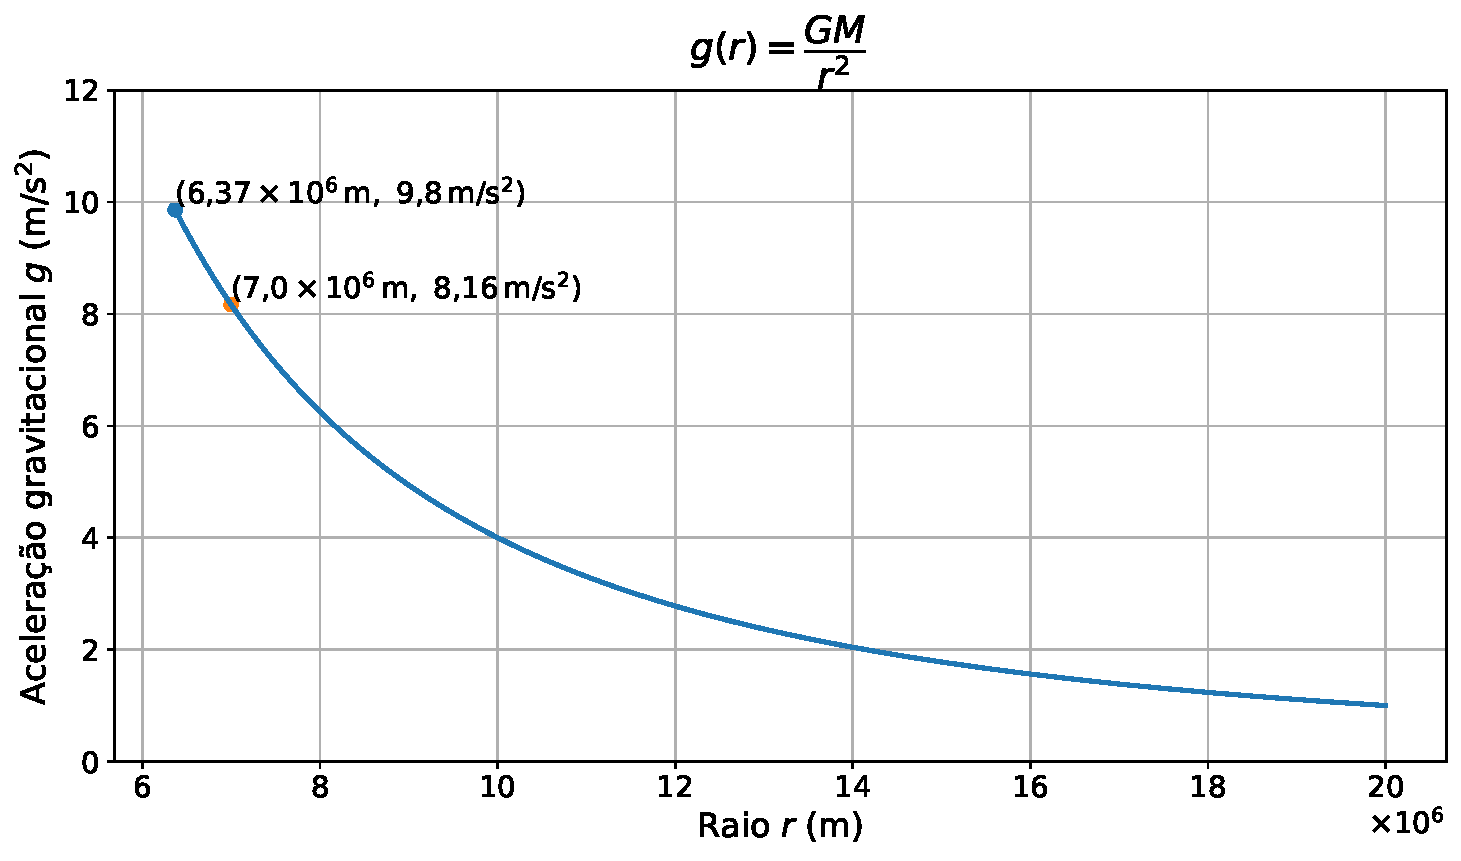
\includegraphics[width=0.9\textwidth]{plots/grafico_gravidade.pdf}
    \caption{Gravidade terrestre em fun\c{c}\~ao da distancia da massa m ao centro da terra.}
    \label{fig:terra_lua}
\end{figure}

\subsubsection*{Cálculo da aceleração da gravidade na distância da Lua}

A aceleração da gravidade é dada por:

\[
g = \frac{GM}{r^2}
\]

Onde:
\begin{itemize}
    \item $G = 6{,}67 \times 10^{-11} \, \text{N·m}^2/\text{kg}^2$
    \item $M = 5{,}97 \times 10^{24} \, \text{kg}$
    \item $r = 384.000 \, \text{km} = 3{,}84 \times 10^8 \, \text{m}$
\end{itemize}

Substituindo os valores:

\[
g = \frac{6{,}67 \times 10^{-11} \cdot 5{,}97 \times 10^{24}}{(3{,}84 \times 10^8)^2}
\]

Calculando:

\[
g \approx 2{,}7 \times 10^{-3} \, \text{m/s}^2
\]

\textbf{Conclusão:}

A aceleração da gravidade da Terra na distância da Lua é aproximadamente:

\[
g \approx 0{,}0027 \, \text{m/s}^2
\]

\begin{itemize}
    \item A gravidade da Terra lá é cerca de 3600 vezes menor,
    \item Mesmo assim, é suficiente para manter a Lua em órbita.
\end{itemize}

\newpage

\subsubsection{(Avançado) Determine a massa da Terra sabendo que $g=9{,}8\,m/s^2$ e $r=6{,}37 \times 10^6\,m$.}
{\color{blue}
\textbf{Resolução:}

Partimos da expressão da aceleração gravitacional:
\[
g = G \frac{M}{r^2}
\]

Isolando a massa $M$:
\[
M = \frac{g\,r^2}{G}
\]

Substituindo os valores:
\[
M = \frac{9{,}8 \cdot (6{,}37 \times 10^6)^2}{6{,}67 \times 10^{-11}}
\]

\[
M = \frac{9{,}8 \cdot (4{,}06 \times 10^{13})}{6{,}67 \times 10^{-11}}
\]

\[
M = \frac{3{,}98 \times 10^{14}}{6{,}67 \times 10^{-11}}
\]

\[
M \approx 5{,}97 \times 10^{24}\,kg
\]

}
\newpage

%==================================================
\section{Trabalho e Energia}

\subsection{Trabalho de uma força constante}
\[
\tau = F \cdot d \cdot \cos\theta
\]

\textbf{Exemplo:} Um operário aplica força de $50\,N$ horizontalmente por $2\,m$:
\[
\tau = 50 \times 2 \times \cos0^\circ = 100\,J
\]

\subsection{Energia Cinética e Potencial}
\[
E_c = \frac{mv^2}{2}, \qquad E_p = mgh
\]

\subsection{Teorema da Energia Cinética}
O trabalho total realizado sobre um corpo é igual à variação da sua energia cinética:
\[
\tau_R = \Delta E_c
\]

\subsection{Exercícios}
\begin{enumerate}
\item Calcule o trabalho realizado por uma força de $10\,N$ ao deslocar um corpo por $3\,m$.
\item Um corpo de $2\,kg$ tem $v=3\,m/s$. Determine sua energia cinética.
\item Um corpo de $5\,kg$ é elevado a $2\,m$. Calcule a energia potencial gravitacional.
\item Um corpo de $1\,kg$ tem $v_0=0$ e sofre força resultante de $10\,N$ por 2 m. Determine $v$.
\item (Avançado) Um bloco desliza plano horizontal ($\mu=0{,}2$). Determine o trabalho da força de atrito em 10 m, se $N=50\,N$.
\end{enumerate}

%==================================================
\section{Sistemas Conservativos e Não Conservativos}

\subsection{Conservação da Energia Mecânica}
Em sistemas sem atrito:
\[
E_m = E_c + E_p = \text{constante}
\]

\textbf{Exemplo:} Um corpo cai de $h=10\,m$:
\[
E_p = E_c \Rightarrow mgh = \frac{mv^2}{2} \Rightarrow v = \sqrt{2gh} = 14\,m/s
\]

\subsection{Sistemas Não Conservativos}
Quando há atrito ou resistência do ar, parte da energia mecânica é transformada em calor.

\subsection{Exercícios}
\begin{enumerate}
\item Um corpo cai de $h=5\,m$. Calcule a velocidade ao atingir o solo (sem atrito).
\item Um corpo é lançado verticalmente com $v_0=20\,m/s$. Determine a altura máxima.
\item Um corpo desliza com atrito ($\mu=0{,}1$) por 10 m. Calcule a energia dissipada.
\item (Intermediário) Em um plano inclinado sem atrito, calcule a velocidade após descer $h=3\,m$.
\item (Avançado) Um pêndulo de $2\,m$ é solto a partir do repouso. Determine a velocidade no ponto mais baixo.
\end{enumerate}

%==================================================
\newpage
\section{Resoluções dos Exercícios}

\subsection{Cinemática}
\begin{enumerate}
\item $s = s_0 + v_0t + \frac{at^2}{2} \Rightarrow 100 = 0 + 0 + \frac{a(10)^2}{2} \Rightarrow a = 2\,m/s^2$
\item $v = \frac{\Delta s}{\Delta t} \Rightarrow 72\,km/h = 20\,m/s \Rightarrow t = \frac{150000}{20} = 7500\,s = 2{,}08\,h$
\item $v = v_0 + at = 5 + 2 \times 6 = 17\,m/s$
\item $s = \frac{at^2}{2} = \frac{3(4)^2}{2} = 24\,m$
\item $v = 0 = 10 + (-a)5 \Rightarrow a=2\,m/s^2$, então $\Delta s = v_0t + \frac{at^2}{2} = 10(5) - \frac{2(5)^2}{2}=25\,m$
\end{enumerate}

\subsection{Leis de Newton}
\begin{enumerate}
\item $a = \frac{F}{m} = \frac{20}{4} = 5\,m/s^2$
\item $F = ma = 1000 \times 2 = 2000\,N$
\item $F_R = 40 - 10 = 30\,N \Rightarrow a = 30/10 = 3\,m/s^2$
\item $F = ma \Rightarrow 5 = 2a \Rightarrow a = 2{,}5\,m/s^2$, $v = v_0 + at = 0 + 2{,}5 \times 3 = 7{,}5\,m/s$
\item $F_R = ma + F_{at}$, $F_{at} = \mu N = 0{,}2 \times 5 \times 9{,}8 = 9{,}8\,N$, $F = 5 \times 2 + 9{,}8 = 19{,}8\,N$
\end{enumerate}

\subsection{Gravitação}
\begin{enumerate}
\item $F = 6{,}67\times10^{-11} \frac{5\times5}{2^2} = 4{,}17\times10^{-10}\,N$
\item $P = mg = 80 \times 9{,}8 = 784\,N$
\item Terra: $98\,N$; Lua: $16\,N$
\item $g = G\frac{M_T}{r^2}$, substituindo dados conhecidos de $G$ e $M_T$, $g \approx 9{,}8\,m/s^2$
\item $M_T = \frac{gr^2}{G} = \frac{9{,}8(6{,}37\times10^6)^2}{6{,}67\times10^{-11}} = 5{,}97\times10^{24}\,kg$
\end{enumerate}

\subsection{Trabalho e Energia}
\begin{enumerate}
\item $\tau = 10\times3\times\cos0 = 30\,J$
\item $E_c = \frac{2(3)^2}{2} = 9\,J$
\item $E_p = 5\times9{,}8\times2 = 98\,J$
\item $\tau = Fd = 10\times2 = 20 = \frac{1}{2}m(v^2 - v_0^2)$ $\Rightarrow v = \sqrt{40} = 6{,}32\,m/s$
\item $W_{at} = -F_{at}d = -\mu N d = -0{,}2\times50\times10 = -100\,J$
\end{enumerate}

\subsection{Sistemas Conservativos}
\begin{enumerate}
\item $v = \sqrt{2gh} = \sqrt{2\times9{,}8\times5} = 9{,}9\,m/s$
\item $v^2 = v_0^2 - 2gh \Rightarrow 0 = 20^2 - 2(9{,}8)h \Rightarrow h = 20{,}4\,m$
\item $E_d = \mu N d = 0{,}1\times10m\times9{,}8=9{,}8\,J$
\item $v = \sqrt{2gh} = \sqrt{2\times9{,}8\times3} = 7{,}7\,m/s$
\item $v = \sqrt{2gh} = \sqrt{2\times9{,}8\times2} = 6{,}26\,m/s$
\end{enumerate}

%%%%%%%% Bibliography 
% Os comandos para incluir as referências bibliográficas
\printingbibliography

\end{document}
